\chapter{Analytic Solutions to the Neutron Diffusion Equation}
\label{ap:analyticSolutions}

\section{Introduction}
  The following are analytic solutions designed for code verification of
  one-dimensional, two-dimensional, and three-dimensional numerical solvers for
  the multigroup neutron diffusion equation. One-group and two-group problems
  are addressed.
  
  For the one-group reference problems, the neutron diffusion problem is written
  \begin{equation} 
    \label{eq:onegroup}
    -D \grad^2 \phi + \Sigma_r \phi =  \frac{1}{\keff} \nu \Sigma_f \phi + 
      q_{fixed}
  \end{equation}
  where
  \begin{conditions}
    D & diffusion coefficient \units{cm}, \\
    \phi & scalar neutron flux \units{$\frac{1}{\text{cm}^2 \; \text{s}}$}, \\
    \Sigma_r & macroscopic removal cross section \units{$\frac{1}{\text{cm}}$},\\
    \keff & effective neutron multiplication factor,\\
    \nu\Sigma_f & number of fission neutrons per unit neutron flux
      \units{$\frac{1}{\text{cm}}$}, \\
    q_{fixed} & fixed volumetric neutron source 
      \units{$\frac{1}{\text{cm}^3 s}$},
  \end{conditions}
   and $\grad^2 \phi = \grad \cdot (\grad \phi)$ is used to simplify notation.
   \eref{eq:onegroup} is valid for problems with constant coefficients
   (homogeneous materials). For problems considered here, material properties
   such as $D$ are constant in some region, either the entire problem or a
   finite subdomain.
  
  For two-group neutron diffusion problems, the two-group neutron diffusion 
  equation is written 
  \begin{align} 
    \label{eq:twogroup1}
    -D_1 \grad^2 \phi_1 + \Sigma_{r1} \phi_1 &= \frac{1}{\keff} \left(
      \nu \Sigma_{f1} \phi_1 + \nu \Sigma_{f2} \phi_2 \right), \\
    \label{eq:twogroup2}
    -D_2 \grad^2 \phi_2 + \Sigma_{r2} \phi_2 &= 
      \Sigma_{s 1 \rightarrow 2} \phi_1,
  \end{align}
  where notation is the same as \eref{eq:onegroup} with the addition of
  subscripts indicating the energy groups and $\phi_1$ is the higher energy 
  group and $\phi_2$ is the lower energy group such that $E_1 > E_2$. This 
  formulation assumes all fission neutrons are created in the high energy group 
  ($\chi_1 = 1$ and $\chi_2 = 0$) and there is no scattering that results in an 
  increase in neutron energy; i.e., no up-scattering 
  ($\Sigma_{s 2 \rightarrow 1} = 0$). These are realistic assumptions for 
  typical diffusive neutron systems.

  Analytic solutions are provided herein. One-dimensional problems can be 
  replicated in a two-dimensional solver using a square geometry and select 
  boundary conditions. To reduce the dimensional of a quadrilateral, two of the 
  boundary conditions are set to mirror flux conditions and two are set to 
  zero-flux $(\phi = 0)$ conditions. For true two-dimensional and three-dimensional 
  problems, all of the boundary conditions are set to zero-flux conditions.
  
  These formulae are common to second order partial differential equations, but
  the formulation here is based in part from Lewis \cite{textbooklewis}.

\section{One-Dimension, One-Group, Fixed Source}
  \label{sec:deriv_1dfixedsrc}
  This one-dimensional problem is in the domain $x \in [0,L_x]$. The material is
  homogeneous within the problem and has fixed coefficient properties.
  The diffusion equation for this problem is 
  \begin{equation}
    \label{eq:1dfixed}
    -D \frac{d^2}{dx^2} \phi(x) + \Sigma_r \phi(x) = q_{fixed}
  \end{equation}
  with boundary conditions specified as
  \begin{align}
    \label{eq:1dfixed_bc1}
    \phi(0) &= 0, \\
    \label{eq:1dfixed_bc2}
    \phi(L_x) &= 0.
  \end{align}
  \eref{eq:1dfixed} can be rewritten as
  \begin{equation}
    \label{eq:1dfixed_buckle}
    \frac{d^2}{dx^2} \phi(x) - \kappa^2 \phi(x) = - \frac{q_{fixed}}{D}
  \end{equation}
  Where $\kappa$ is a shape term and is given for this problem as
  \begin{equation}
    \label{eq:1dfixed_b2}
    \kappa^2 = \frac{\Sigma_r}{D}.
  \end{equation}
  Begin by allowing the solution to be composed of homogeneous and particular
  solutions. 
  \begin{equation} 
    \phi(x) = \phi_H(x) + \phi_P(x)
  \end{equation}
  Using the form of \eref{eq:1dfixed_buckle}, the homogeneous solution satisfies 
  \begin{equation}
    \label{eq:1dfixed_homog}
    \frac{d^2}{dx^2} \phi_H(x) - \kappa^2 \phi_H(x) = 0.
  \end{equation}
  The homogeneous solution $\phi_H(x)$ has form 
  \begin{equation}
    \label{eq:1dfixed_homog_form}
    \phi_H(x) = c_1 \, \cosh(\kappa \, x) + c_2 \, \sinh(\kappa \, x)
  \end{equation}
  where $c_1$ and $c_2$ are unknown constants.
  The particular solution is given for a constant value $q_{fixed}$.
  \begin{equation}
    \label{eq:1dfixed_particular}
    \phi_P(x) = \frac{q_{fixed}}{D\,\kappa^2}.
  \end{equation}
  Combining the homogeneous and particular solutions.
  \begin{equation}
    \label{eq:1dfixed_constants}
    \phi(x) = c_1 \, \cosh(\kappa \, x) + c_2 \, \sinh(\kappa \, x) +
      \frac{q_{fixed}}{D\,\kappa^2}
  \end{equation}
  Next, boundary conditions are considered to solve for the unknown coefficients
  in \eref{eq:1dfixed_constants}. Beginning with the boundary at $x=0$ as 
  specified in \eref{eq:1dfixed_bc1}.
  \begin{align}
    \phi(0) &= 0 \\
    &= c_1 + \frac{q_{fixed}}{D\,\kappa^2} \\
    \label{eq:1dfixed_c1}
    \therefore \; c_1 &= - \frac{q_{fixed}}{D\,\kappa^2}
  \end{align}
  \eref{eq:1dfixed_c1} is then inserted into \eref{eq:1dfixed_constants}.
  \begin{align}
    \phi(x) &= -\frac{q_{fixed}}{D\,\kappa^2} \, \cosh(\kappa \, x) + c_2 \,
      \sinh(\kappa \, x) + \frac{q_{fixed}}{D\kappa^2} \\
    \phi(x) &= \frac{q_{fixed}}{D\,\kappa^2} \left( 1- \cosh(\kappa \, x)  
      \right) + c_2 \, \sinh(\kappa \, x)
  \end{align}
  The next boundary condition is evaluated at $x=L_x$ as specified in
  \eref{eq:1dfixed_bc2}.
  \begin{align}
    \phi(L_x) &= 0 \\
    &= \frac{q_{fixed}}{D\,\kappa^2} \left( 1- \cosh(\kappa \, L_x )  \right) + 
      c_2 \, \sinh(\kappa \, L_x) \\
    \label{eq:1dfixed_c2}
    \therefore c_2 &= \frac{\frac{q_{fixed}}{D\,\kappa^2} 
      \left(\cosh(\kappa \, L_x) - 1 \right)} {\sinh(\kappa \, L_x)}
  \end{align}
  All constants of the problem are now specified in \eref{eq:1dfixed_c1} and 
  \eref{eq:1dfixed_c2} and can be substitued into \eref{eq:1dfixed_constants}.
  \begin{equation}
    \label{eq:analytic_1dfixedsrc}
    \phi(x) = \left( \frac{q_{fixed}}{D} \right) 
      \left( 1-\cosh(\kappa\,x) +
      \frac{\cosh(\kappa\,L_x)-1}{\sinh(\kappa\,L_x)}
      \sinh(\kappa\,x)\right)
  \end{equation}
  Recall $\kappa^2 = \frac{\Sigma_r}{D}$ as in \eref{eq:1dfixed_b2}. A typical 
  result of \eref{eq:analytic_1dfixedsrc} is presented in
  \fref{fig:fixed_critical}. Note that the magnitude of the function is not
  arbitrary and is specified by the magnitude of the external source
  $q_{fixed}$.

  \begin{figure}
    \centering
    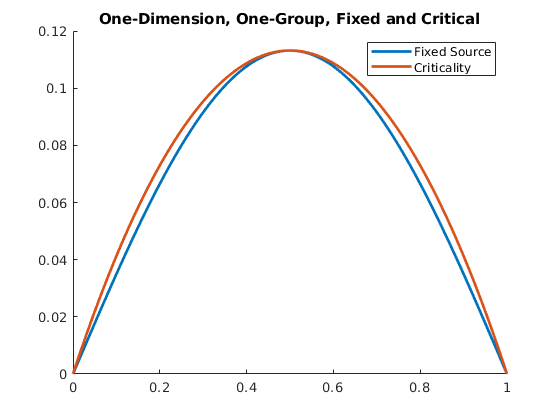
\includegraphics[width=0.7\textwidth]{fixed_critical}
    \caption{Fixed Source and Criticality Flux Shapes for One-Dimension,
      One-Group Problems.}
    \label{fig:fixed_critical}
  \end{figure}
  
\section{One-Dimension, One-Group, Criticality} 
  \label{sec:deriv_1d1g}
  This one-dimensional problem is in the domain $x \in [0,L_x]$. The material
  is homogeneous within the problem and has fixed coefficient properties. The
  diffusion equation for this problem is
  \begin{equation}
    \label{eq:1d1g}
    -D \frac{d^2}{dx^2} \phi(x) + \Sigma_r \phi(x) = 
      \frac{1}{\keff} \nu \Sigma_f \phi(x)
  \end{equation}
  with boundary conditions
  \begin{align}
    \label{eq:1d1g_bc1}
    \phi(0) &= 0 ,\\
    \label{eq:1d1g_bc2}
    \phi(L_x) &= 0.
  \end{align}
  \eref{eq:1d1g} can be rewritten as
  \begin{equation}
    \label{eq:1d1g_buckle}
    \frac{d^2}{dx^2} \phi(x) + B^2 \phi(x) = 0
  \end{equation}
  where $B$ is the buckling term defined as
  \begin{equation}
    \label{eq:1d1g_b2}
    B^2 = \frac{\frac{1}{\keff} \nu \Sigma_f - \Sigma_r}{D}.
  \end{equation}
  \eref{eq:1d1g_buckle} has general solution 
  \begin{equation}
    \label{eq:1d1g_general}
    \phi(x) = c_1 \, \cos(B \, x) + c_s \, \sin(B \, x)
  \end{equation}
  where $c_1$ and $c_2$ are unknown constants.
  Using \eref{eq:1d1g_general}, the first boundary condition is applied at $x=0$
  as specified in \eref{eq:1d1g_bc1}.
  \begin{align}
    \phi(0) &= 0 \\
    &= c_1 \\
    \label{eq:1d1g_c1}
    \therefore \; c_1 &= 0
  \end{align}
  \eref{eq:1d1g_c1} is then inserted into \eref{eq:1d1g_general}, giving
  \begin{equation}
    \label{eq:1d1g_sin}
    \phi(x) = c_2 \, \sin(B \, x).
  \end{equation}
  Next, the second boundary condition is evaluated at $x=L_x$ as specified in
  \eref{eq:1d1g_bc2}.
  \begin{align}
    \phi(L_x) &= 0 ,\\
    &= c_2 \, \sin(B \, L_x).
  \end{align}
  For a non-trivial solution, this problem is an eigenvalue problem with $B$
  determined by the boundary condition such that 
  \begin{equation}
    0 = \sin(B_g \, L_x)
  \end{equation}
  where $B_g$ is the geometric buckling which is specified by the geometry of
  the problem. This term is only zero for specific values of $B_g$.
  This implies $c_2$ is arbitrary and the
  magnitude of the flux can be normalized to a constant. For simplicity, allow
  $c_2 = \phi_0$. Then, noting the zeros of the sine function.
  \begin{align}
    B_g \, L_x &= n \, \pi, \\
    B_g &= \frac{n \, \pi}{L_x},
  \end{align}
  where $n$ is an integer. For the fundamental mode, $n=1$,
  \begin{equation}
    \label{eq:1d1g_buckle_geom}
    B_g = \frac{\pi}{L_x}.
  \end{equation}
  Substitute \eref{eq:1d1g_buckle_geom} into \eref{eq:1d1g_sin} for the solution
  to the fundamental eigenmode.
  \begin{equation}
    \label{eq:analytic_1d1g}
    \phi(x) = \phi_0 \, \sin\left(\frac{\pi}{L_x} x \right)
  \end{equation}
  A typical flux shape is plotted in \fref{fig:fixed_critical} along with the
  solution for a fixed-source problem. Recall that the magnitude is arbitrary so 
  the flux is normalized to have maximum equal to the fixed solution for 
  visualization purposes.
  Recalling the definition of $B$ from \eref{eq:1d1g_b2}, the fundamental
  eigenvalue of the problem, $\keff$, can be solved for by setting buckling
  equal to geometric buckling.
  \begin{align}
    B_g &= B \\
    \left( \frac{\pi}{L_x} \right)^2 &= 
      \frac{\frac{1}{\keff} \nu \Sigma_f - \Sigma_r}{D} \\
    \label{eq:keff1d}
    \keff &= \frac{\nu \Sigma_f}{D \left(\frac{\pi}{L_x}\right)^2 + \Sigma_r}
  \end{align}
  For a problem with material cross sections given in \tref{tab:1group_simple}
  and $L_x = 100 \units{cm}$, then the resulting effective multiplication factor
  is
  \begin{equation}
    \keff = 1.998028.
  \end{equation}

  \begin{table}
    \caption{One-Group Sample Cross Sections.}
    \label{tab:1group_simple}
    \begin{center}
      \begin{tabular}{cc}
        \toprule
        Cross Section & Value \\
        \midrule
        $D \units{cm}$ & 1 \\
        $\Sigma_r       \units{$\frac{1}{\text{cm}}$}$& 1 \\
        $\nu \Sigma_{f} \units{$\frac{1}{\text{cm}}$}$& 2 \\
        \bottomrule
      \end{tabular}
    \end{center}
  \end{table}

\section{Two-Dimension, One-Group, Criticality}
  \label{sec:deriv_2d1g}
  This two-dimensional problem is in the rectangular domain $[0,L_x] \times
  [0,L_y]$. That is, $x \in [0,L_x]$ and $y \in [0,L_y]$. The material is
  homogeneous within the problem and has fixed coefficient properties. The
  diffusion equation for this problem is 
  \begin{equation}
    \label{eq:2d1g}
    -D \grad^2 \phi(x,y) + \Sigma_r \phi(x,y) = 
      \frac{1}{\keff} \nu \Sigma_f \phi(x,y)
  \end{equation}
  with boundary conditions
  \begin{align}
    \label{eq:2d1g_bc1}
    \phi(0,y) &= 0 ,\\
    \label{eq:2d1g_bc2}
    \phi(L_x,y) &= 0 ,\\
    \label{eq:2d1g_bc3}
    \phi(x,0) &= 0 ,\\
    \label{eq:2d1g_bc4}
    \phi(x,L_y) &= 0.
  \end{align}
  \eref{eq:2d1g} can be rewritten as
  \begin{equation}
    \label{eq:2d1g_buckle}
    \grad^2 \phi(x,y) + B^2 \phi(x,y) = 0
  \end{equation}
  where $B$ is the buckling term and is given for this problem is given as
  \begin{equation}
    \label{eq:2d1g_b2}
    B^2 = \frac{\frac{1}{\keff} \nu \Sigma_f - \Sigma_r}{D}.
  \end{equation}
  The Laplacian, $\grad^2$, in \eref{eq:2d1g_buckle} for two-dimensional 
  Cartesian geometry is then expanded into partial derivatives as
  \begin{equation}
    \label{eq:2d1g_partial}
    \frac{\partial^2}{\partial x^2} \phi(x,y) + \frac{\partial^2}{\partial y^2}
      \phi(x,y) + B^2 \phi(x,y) = 0.
  \end{equation}
  The method of separation of variables is used to solve
  \eref{eq:2d1g_partial}. Begin by assuming that $\phi(x,y)$ is separable as
  functions of $x$ and $y$.
  \begin{equation}
    \label{eq:2d1g_separable}
    \phi(x,y) = X(x)\,Y(y)
  \end{equation}
  Then, inserting \eref{eq:2d1g_separable} into \eref{eq:2d1g_partial}.
  \begin{align}
    \frac{\partial^2}{\partial x^2} \left( X(x)\,Y(y) \right) + 
      \frac{\partial^2}{\partial y^2} \left( X(x)\,Y(y) \right) + 
      B^2 X(x)\,Y(y) &= 0 \\
    \label{eq:2d1g_above}
    Y(y) \frac{d^2}{d x^2} X(x) + X(x) \frac{d^2}{d y^2} Y(y) + 
      B^2 X(x) \, Y(y) &= 0
  \end{align}
  Each of the derivatives operates on a function of only one variable, so the
  partial derivatives have become standard derivatives. Dividing by the quantity 
  $X(x)\,Y(y)$ yields
  \begin{equation}
    \label{eq:2d1g_divide_sum}
    \frac{1}{X(x)} \, \frac{d^2}{d x^2} X(x) + 
      \frac{1}{Y(y)} \, \frac{d^2}{d y^2} Y(y) + 
      B^2 = 0.
  \end{equation}

  The first two terms of \eref{eq:2d1g_divide_sum} are functions of only $x$ and
  $y$ respectively, and their sum is equal to a constant. Therefore, both of the
  terms must also be equal to a constant \cite{lamarsh1966}. Splitting
  \eref{eq:2d1g_divide_sum} into two equations yields
  \begin{align}
    \label{eq:2d1g_x}
    \frac{1}{X(x)} \, \frac{d^2}{d x^2} X(x) + \alpha^2 &= 0, \\
    \label{eq:2d1g_y}
    \frac{1}{Y(y)} \, \frac{d^2}{d y^2} Y(y) + \beta^2 &= 0,
  \end{align}
  where $\alpha$ and $\beta$ are constants such that
  \begin{equation}
    \label{eq:2d1g_buckle_alphabeta}
    \alpha^2 + \beta^2 = B^2.
  \end{equation}
  Consider \eref{eq:2d1g_x} and boundary conditions specified in
  \eref{eq:2d1g_bc1} and \eref{eq:2d1g_bc2}. Then, \eref{eq:2d1g_x} can be
  rewritten.
  \begin{equation}
    \label{eq:2d1g_xeqn}
    \frac{d^2}{dx^2} X(x) + \alpha^2 X(x) = 0
  \end{equation}
  The form of \eref{eq:2d1g_xeqn} is similar to the previous problem in 
  \eref{eq:1d1g_buckle} which has general solution of the form
  \begin{equation}
    \label{eq:2d1g_x_general}
    X(x) = c_1 \, \cos(\alpha \, x) + c_2 \, \sin(\alpha \, x).
  \end{equation}
  $X(x)$ has solution similar to the form of the one-dimension, one-group,
  criticality problem from \sref{sec:deriv_1d1g} as the boundary conditions are
  similar. Using the method from \sref{sec:deriv_1d1g}, the fundamental mode is
  given as
  \begin{align}
    \label{eq:2d1g_x_alpha}
    \alpha &= \frac{\pi}{L_x}, \\
    \label{eq:2d1g_x_solution}
    X(x) &= \phi_{0,x} \, \sin\left(\frac{\pi}{L_x} x\right),
  \end{align}
  where $\phi_{0,x}$ is an arbitrary constant.
  Similar procedure is performed to solve for $Y(y)$ yielding
  \begin{equation}
    \label{eq:2d1g_y_solution}
    Y(y) = \phi_{0,y} \sin\left(\frac{\pi}{L_y} y \right)
  \end{equation}
  and 
  \begin{equation}
    \label{eq:2d1g_y_beta}
    \beta = \frac{\pi}{L_y}.
  \end{equation}
  \eref{eq:2d1g_x_solution} and \eref{eq:2d1g_y_solution} are substituted into
  \eref{eq:2d1g_separable} giving
  \begin{equation}
    \label{eq:analytic_2d1g}
    \phi(x,y) = \phi_0 \sin\left(\frac{\pi}{L_x} x\right) \, 
      \sin\left(\frac{\pi}{L_y} y\right)
  \end{equation}
  where $\phi_0 = \phi_{0,x} \phi_{0,y}$ and is also arbitrary.
  A typical flux shape given by \eref{eq:analytic_2d1g} is plotted
  in \fref{fig:2d1g}.

  \begin{figure}
    \centering
    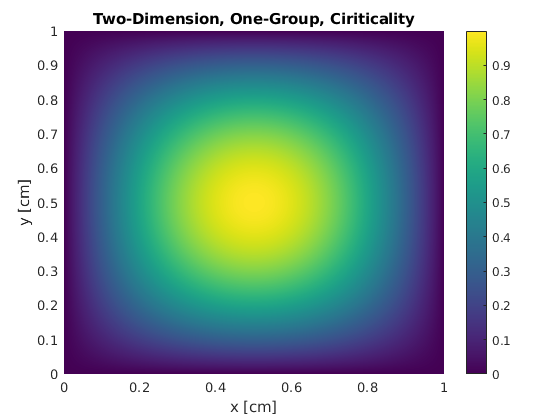
\includegraphics[width=0.7\textwidth]{2d1g}
    \caption{Two-Dimension Criticality Flux Shape.}
    \label{fig:2d1g}
  \end{figure}

  Using \eref{eq:2d1g_buckle_alphabeta} along with \eref{eq:2d1g_x_alpha} and a
  \eref{eq:2d1g_y_beta}, the geometric buckling can be written.
  \begin{equation}
    \label{eq:2d1g_buckle_geom}
    B_g^2 = \left(\frac{\pi}{L_x}\right)^2 + \left(\frac{\pi}{L_y}\right)^2
  \end{equation}
  Setting \eref{eq:2d1g_buckle_geom} equal to \eref{eq:2d1g_b2} yields an
  expression for $\keff$.
  \begin{align}
    \left(\frac{\pi}{L_x}\right)^2 + \left(\frac{\pi}{L_y}\right)^2 &=
      \frac{\frac{1}{\keff} \nu \Sigma_f - \Sigma_r}{D} \\
    \keff &= \frac{\nu \Sigma_f}{D \left( \left(\frac{\pi}{L_x}\right)^2 + 
      \left( \frac{\pi}{L_y}\right)^2 \right) + \Sigma_r}
  \end{align}
  Using the material coefficients specified in \tref{tab:1group_simple}, and
  $L_x=L_y=100 \units{cm}$ gives 
  \begin{equation}
    \label{eq:keff2d}
    \keff = 1.996060.
  \end{equation}
  
\section{One-Dimension, Two-Group, Criticality}
  \label{sec:deriv_1d2g}
  This one-dimensional problem is meant to test the multigroup solution method of
  the solver. The problem is in the domain $x \in [0,L_x]$ and has two energy
  groups. The material is homogeneous within the problem and has fixed
  coefficient properties. With this geometry, \eref{eq:twogroup1} and
  \eref{eq:twogroup2} become
  \begin{align}
    \label{eq:1d2g_1}
    - D_1 \frac{d^2}{dx^2} \phi_1(x) + \Sigma_{r1} \, \phi_1(x) &= 
      \frac{1}{\keff} \left( \nu \Sigma_{f1} \phi_1(x) + \nu \Sigma_{f2}
      \phi_2(x) \right) \\
    \label{eq:1d2g_2}
    -D_2 \frac{d^2}{dx^2} \phi_2(x) + \Sigma_{r2} \phi_2(x) &= 
      \Sigma_{s 1 \rightarrow 2} \phi_1(x)
  \end{align}
  with boundary conditions
  \begin{align}
    \label{eq:1d2g_bc0}
    \phi_g(0) &= 0 ,\\
    \label{eq:1d2g_bcLx}
    \phi_g(L_x) &= 0.
  \end{align}
  
  This is a bare core problem ($\phi=0$ on all boundaries); therefore, the 
  general solution to \eref{eq:1d2g_1} and \eref{eq:1d2g_2} has the form common
  to one-group bare core problems,
  \begin{equation}
    \label{eq:multigroup_buckle}
    \frac{d^2}{dx^2} \phi_g(x) + B^2 \phi_g(x) = 0 \qquad \text{for } g=1,2
  \end{equation}
  where $B$ is a buckling term common to both energy groups (not group
  specific) \cite{textbookhenry}. The general solution to this equation is
  \begin{equation}
    \label{eq:multigroup_general}
    \phi_g(x) = c_{1g} \, \cos(B\,x) + c_{2g} \, \sin(B\,x).
  \end{equation}
  Boundary conditions are applied next. Beginning with the boundary condition at
  $x=0$ as specified in \eref{eq:1d2g_bc0} gives
  \begin{align}
    \phi_g(0) &= 0, \\
    &= c_{1g}, \\
    \label{eq:1d2g_c1g}
    \therefore \; c_{1g} &= 0.
  \end{align}
  Then, using \eref{eq:1d2g_c1g}, \eref{eq:multigroup_general} can be rewritten 
  as
  \begin{equation}
    \label{eq:1d2g_sin}
    \phi_g(x) = c_{2g} \, \sin(B\,x).
  \end{equation}
  For notational clarity, let $k_g = c_{2g}$.
  Evaluating the boundary condition at $x=L_x$ as specified in
  \eref{eq:1d2g_bcLx}.
  \begin{align}
    \phi_g(L_x) &= 0 ,\\
    &= k_g \, \sin(B \, L_x).
  \end{align}
  The buckling $B$ is then specified by the zeros of the sine function. The
  fundamental mode is given.
  \begin{equation}
    \label{eq:1d2g_buckle_geom}
    B = \frac{\pi}{L_x}
  \end{equation}
  To find the unknown coefficients $k_g$, differentiate \eref{eq:1d2g_sin}
  twice with respect to $x$.
  \begin{equation}
    \label{eq:1d2g_sin_d2}
    \frac{d^2}{dx^2} \phi_g(x) = - B^2 \, k_g \, \sin(B\,x)
  \end{equation}
  Insert \eref{eq:1d2g_sin} and \eref{eq:1d2g_sin_d2} into \eref{eq:1d2g_1} and
  \eref{eq:1d2g_2}.
  \begin{align}
    D_1 \, B^2 \, k_1 \, \sin(B\,x) + \Sigma_{r1} \, k_1 \, \sin(B\,x) &=
      \frac{1}{\keff} \left( \nu \Sigma_{f1} \, k_1 \, \sin(B \, x) + \nu
      \Sigma_{f2} \, k_2 \, \sin(B\,x) \right) \\
    D_2 \, B^2 \, k_2 \sin(B\,x) + \Sigma_{r2} \, k_2 \, \sin(B\,x) &=
      \Sigma_{s 1\rightarrow 2} \, k_1 \, \sin(B\,x)
  \end{align}
  Dividing through the equations by $\sin(B\,x)$.
  \begin{align}
    \label{eq:1d2g_expression1}
    D_1 \, B^2 \,k_1+ \Sigma_{r1}\,k_1 &= \frac{1}{\keff} \left( \nu \Sigma_{f1}
      \, k_1 + \nu \Sigma_{f2} \, k_2 \right) \\
    \label{eq:1d2g_expression2}
    D_2 \, B^2 \, k_2 + \Sigma_{r2}\,k_2 &= \Sigma_{s 1\rightarrow 2} \, k_1
  \end{align}
  Beginning with \eref{eq:1d2g_expression2} and solving for the quantity
  $\frac{k_2}{k_1}$ and recalling \eref{eq:1d2g_buckle_geom}.
  \begin{align}
    \frac{k_2}{k_1} &= \frac{\Sigma_{s 1\rightarrow 2}}{D_2 \, B^2 + \Sigma_{r2}}
      \\
    \label{eq:1d2g_ratio}
    \frac{k_2}{k_1} &= \frac{\Sigma_{s 1\rightarrow 2}}{D_2 \,
      \left(\frac{\pi}{L_x}\right)^2 + \Sigma_{r2}}
  \end{align}
  The quantity $\frac{k_2}{k_1}$ relates the magnitudes of $\phi_1(x)$ and
  $\phi_2(x)$. The relative magnitude is not arbitrary as expressed in
  \eref{eq:1d2g_ratio} but $k_1$ is arbitrary. Allow $k_1 = \phi_0$ where
  $\phi_0$ is an arbitrary constant.

  Returning to \eref{eq:1d2g_expression1} and solving for the eigenvalue
  $\keff$.
  \begin{align}
    \keff &= \frac{\nu \Sigma_{f1} \, k_1 + \nu \Sigma_{f2} \, k_2}
      {D_1 \, B^2 k_1 + \Sigma_{r1} \, k_1 }\\
    \keff &= \frac{\nu \Sigma_{f1} \, k_1 + \nu \Sigma_{f2} \, k_2}
      {D_1 \, \left(\frac{\pi}{L_x}\right)^2 \, k_1 + \Sigma_{r1} \, k_1}
  \end{align}
  Divide the top and bottom of the ratio by $k_1$.
  \begin{equation}
    \label{eq:1d2g_keff}
    \keff = \frac{\nu \Sigma_{f1} + \nu \Sigma_{f2} \, \frac{k_2}{k_1}}
      {D_1 \, \left(\frac{\pi}{L_x}\right)^2 + \Sigma_{r1}}
  \end{equation}
  Recalling the quantity $\frac{k_2}{k_1}$ from \eref{eq:1d2g_ratio}.

  The flux shape for $\phi_1(x)$ and $\phi_2(x)$ are given by combining
  \eref{eq:1d2g_sin}, \eref{eq:1d2g_buckle_geom}, and \eref{eq:1d2g_ratio}.
  Combining these equations and rewriting yields
  \begin{align}
    \phi_1(x) &= \phi_0 \, \sin\left(\frac{\pi}{L_x} x \right), \\
    \phi_2(x) &= \frac{k_2}{k_1} \, \phi_0 \, \sin\left(\frac{\pi}{L_x} x
      \right),
  \end{align}
  recalling $\phi_0$ is an arbitrary constant.
  An example solution is plotted in \fref{fig:1d2g}. The ratio
  $\frac{k_2}{k_1}$ is given in \eref{eq:1d2g_ratio}.
  Finally, $\keff$ is given in \eref{eq:1d2g_keff}. The cross sections from 
  VVER440 benchmark, material MAT1, described in \sref{sec:vver440} are used for
  this problem. For ease of reference, the cross sections are also presented in 
  \tref{tab:1d2g_vver440}. For the specified cross sections and 
  $L_x = 100 \units{cm}$, the solutions are
  \begin{align}
    \frac{k_2}{k_1} &= 0.0261324, \\
    \keff &= 0.892349.
  \end{align}

  \begin{figure}
    \centering
    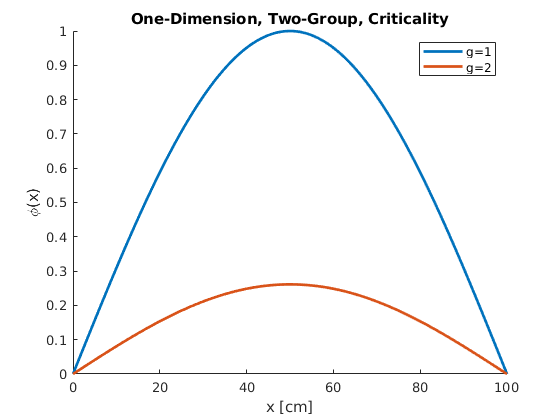
\includegraphics[width=0.7\textwidth]{1d2g}
    \caption{Example Two-Group Flux Plot.}
    \label{fig:1d2g}
  \end{figure}

  \begin{table}
    \caption{Two-Group VVER440 Material Constants.}
    \label{tab:1d2g_vver440}
    \begin{center}
      \begin{tabular}{cr}
        \toprule
        & MAT1 \\
        \midrule
        $D_1 \units{cm}$ & 1.3466E+00 \\
        $D_2 \units{cm}$ & 3.7169E-01 \\
        $\Sigma_{r1} \units{$\frac{1}{\text{cm}}$}$ & 2.5255E-02 \\
        $\Sigma_{r2} \units{$\frac{1}{\text{cm}}$}$ & 6.4277E-02 \\
        $\Sigma_{s 1 \rightarrow 2} \units{$\frac{1}{\text{cm}}$}$ &
           1.6893E-02 \\
        $\nu \Sigma_{f1} \units{$\frac{1}{\text{cm}}$}$ & 4.4488E-03 \\
        $\nu \Sigma_{f2} \units{$\frac{1}{\text{cm}}$}$ & 7.3753E-02 \\
        \bottomrule
      \end{tabular}
    \end{center}
  \end{table}

\section{One-Dimension, One-Group, Two Region, Criticality}
  \label{sec:deriv_2reg}
  This one-dimensional problem is meant to simulate a reactor with non-fissile,
  reflective material at the edge of the reactor. The purpose of this problem is
  to test the materials mapping of a multigroup neutron diffusion solver. The
  problem is in the domain $x \in [0,L_R]$. Geometry is shown in
  \fref{fig:2reg_geom}. Fuel material (subscript F) is located in $x \in
  [0,L_F]$ and reflector material (subscript R) is located in $ x \in
  [L_F,L_R]$. The material is homogeneous within each respective section, and
  has fixed coefficient properties in each region.  The diffusion equation for
  this problem is 
  \begin{align}
    \label{eq:2regF}
    -D_F \frac{d^2}{dx^2} \phi_F(x) + \Sigma_{rF} \phi_F(x) &= \frac{1}{\keff} 
      \nu \Sigma_{fF} \phi_F(x) \quad \forall \; x \in [0,L_F] \\
    \label{eq:2regR}
    -D_R \frac{d^2}{dx^2} \phi_R(x) + \Sigma_{rR} \phi_R(x) &= 0  
      \qquad \qquad \qquad \forall \; x \in [L_F,L_R]
  \end{align}
  with boundary and interfacial conditions
  \begin{align}
    \label{eq:2reg_bc0}
    \left. \frac{d}{dx} \phi_F(x) \right|_{x=0} &= 0, \\
    \label{eq:2reg_flux_continuity}
    \phi_F(L_F) &= \phi_R(L_F) ,\\
    \label{eq:2reg_current_continuity}
    D_F \left. \frac{d}{dx} \phi_F(x) \right|_{x=L_F} &= 
      D_R \left. \frac{d}{dx} \phi_R(x) \right|_{x=L_F} ,\\
    \label{eq:2reg_bcLR}
    \phi_R(L_R) &= 0.
  \end{align}
  \begin{figure}
    \centering
    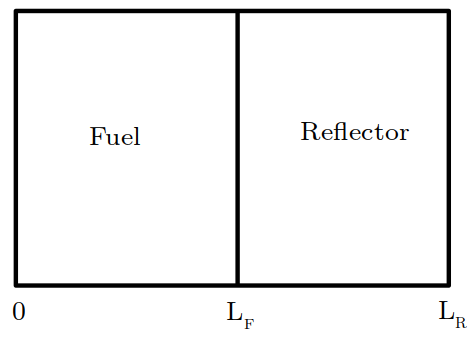
\includegraphics[width=0.5\textwidth]{2reg_geom}
    \caption{Geometry for Two Region Problem.}
    \label{fig:2reg_geom}
  \end{figure}

  Beginning in the fueled region, the diffusion equation in \eref{eq:2regF} can 
  be rewritten with a fuel buckling term $B_F$ as
  \begin{equation}
    \label{eq:2regF_buckle}
    \frac{d^2}{dx^2} \phi_F(x) + B_F^2 \phi_F(x) = 0 
  \end{equation}
  where $B_F^2$ is the buckling term in the fuel and is given by
  \begin{equation}
    \label{eq:2regF_b2}
    B_F^2 = \frac{\frac{1}{\keff} \nu \Sigma_{fF} - \Sigma_{rF}}{D_F}.
  \end{equation}
  \eref{eq:2regF_buckle} has general solution of the form
  \begin{equation}
    \label{eq:2regF_general}
    \phi_F(x) = c_{1F} \, \cos(B_F\,x) + c_{2F} \, \sin(B_F\,x)
  \end{equation}
  where $c_{1F}$ and $c_{2F}$ are unknown constant coefficients.
  The derivative of \eref{eq:2regF_general} is also provided as it will be
  useful for evaluating boundary and interface conditions.
  \begin{equation}
    \label{eq:2regF_general_derivative}
    \frac{d}{dx}\phi_F(x) = -c_{1F} \, B_F \, \sin(B_F\,x) + 
      c_{2F} \, B_F \, \cos(B_F\,x)
  \end{equation}
  Using \eref{eq:2regF_general_derivative}, the boundary condition is evaluated
  at $x=0$ as specified in \eref{eq:2reg_bc0}.
  \begin{align}
    \left. \frac{d}{dx} \phi_F(x) \right|_{x=0} &= 0, \\
    &= c_{2F} \, B_F, \\
    \label{eq:2reg_c2f}
    \therefore \; c_{2F} &= 0.
  \end{align}
  \eref{eq:2reg_c2f} is inserted into \eref{eq:2regF_general} yielding
  \begin{equation}
    \label{eq:2regF_cos}
    \phi_F(x) = c_{1F} \, \cos(B_F\, x)
  \end{equation}
  and its derivative is also provided
  \begin{equation}
    \label{eq:2regF_cos_derivative}
    \frac{d}{dx} \phi_F(x) = -c_{1F} \, B_F \, \sin(B_F \, x).
  \end{equation}

  Next, the reflector region is considered as in \eref{eq:2regR}. This equation
  can be rewritten as
  \begin{equation}
    \label{eq:2regR_buckle}
    \frac{d^2}{dx^2} \phi_R(x) - \kappa_R^2 \phi_R(x) = 0
  \end{equation}
  where $\kappa_R^2$ is the shape term in the reflector and is given as
  \begin{equation}
    \label{eq:2regR_b2}
    \kappa_R^2 = \frac{\Sigma_{rR}}{D_R}.
  \end{equation}
  \eref{eq:2regR_buckle} has general solution of the form
  \begin{equation}
    \label{eq:2regR_general}
    \phi_R(x) = c_{1R} \, \cosh(\kappa_R\, (x-L_F)) + c_{2R} \, 
      \sinh(\kappa_R\,(x-L_F))
  \end{equation}
  where $c_{1R}$ and $c_{2R}$ are unknown constant coefficients.
  Note the use of $(x-L_F)$ instead of $x$ in \eref{eq:2regR_general}. This
  choice is valid because hyperbolic cosine and hyperbolic sine can be rewritten
  as exponential functions and the subtraction in the argument is equivalent to
  multiplication by a constant.
  The derivative of \eref{eq:2regR_general} is also provided as it will be
  useful for evaluating boundary conditions.
  \begin{equation}
    \label{eq:2regR_general_derivative}
    \frac{d}{dx} \phi_R(x) = c_{1R} \, \kappa_R \, \sinh(\kappa_R \, (x-L_F)) + 
      c_{2R} \, \kappa_R \, \cosh(\kappa_R \, (x-L_F))
  \end{equation}
  The zero-flux boundary condition at $x=L_R$ is treated as specified in
  \eref{eq:2reg_bcLR}.
  \begin{align}
    \phi_R(L_R) &= 0 \\
    &= c_{1R} \, \cosh(\kappa_R \, (L_R - L_F)) + c_{2R} \sinh(\kappa_R \, (L_R-L_F))
  \end{align}
  Then, solving for $c_{2R}$.
  \begin{align}
    c_{2R} &= \frac{-c_{1R}\,\cosh(\kappa_R\,(L_R - L_F))}{\sinh(\kappa_R \,(L_R-L_F))} \\
    \label{eq:2reg_c2r_a}
    c_{2R} &= -c_{1R} \frac{1}{\tanh(\kappa_R\,(L_R-L_F))}
  \end{align}

  Next, the current continuity condition at $x=L_F$ is considered as specified
  in \eref{eq:2reg_current_continuity}. \eref{eq:2regF_cos_derivative} and
  \eref{eq:2regR_general_derivative} are used to evaluate the functions.
  Evaluating the boundary condition yields
  \begin{align}
    \left. D_F \frac{d}{dx} \phi_F(x) \right|_{x=L_F} &= 
      \left. D_R \frac{d}{dx} \phi_R(x) \right|_{x=L_F} ,\\
    -D_F \, c_{1F} \, B_F \, \sin(B_F \, L_F) &= D_R \, \kappa_R \, c_{2R}.
  \end{align}
  Then, solving for $c_{2R}$ gives
  \begin{equation}
    \label{eq:2reg_c2r_b}
    c_{2R} = \frac{-D_F \, c_{1F} \, B_F \, \sin(B_F \, L_F)}{D_R\,\kappa_R}.
  \end{equation}
  Next, the flux continuity condition at $x=L_F$ is considered as specified in 
  \eref{eq:2reg_flux_continuity}. \eref{eq:2regF_cos} and 
  \eref{eq:2regR_general} are used to evaluate the functions as
  \begin{align}
    \phi_F(L_F) &= \phi_R(L_F) ,\\
    c_{1F} \, \cos(B_f \, L_F) &= c_{1R} ,\\
    \label{eq:2reg_c1r}
    c_{1R} &= c_{1F} \, \cos(B_F \, L_F).
  \end{align}

  Now the constant coefficients $c$ are solved. Setting \eref{eq:2reg_c2r_a} 
  equal to \eref{eq:2reg_c2r_b} gives
  \begin{align}
    -c_{1R} \frac{1}{\tanh(\kappa_R\,(L_R-L_F))}
      &= \frac{-D_F \, c_{1F} \, B_F \, \sin(B_F \, L_F)}{D_R\,\kappa_R}, \\
    c_{1R} \frac{1}{\tanh(\kappa_R\,(L_R-L_F))}
      &= \frac{D_F \, c_{1F} \, B_F \, \sin(B_F \, L_F)}{D_R\,\kappa_R}.
  \end{align}
  Inserting the expression for $c_{1R}$ from \eref{eq:2reg_c1r}.
  \begin{equation}
    \label{eq:2reg_c1f_arbitrary}
    \frac{c_{1F} \, \cos(B_F \, L_F)}{\tanh(\kappa_R \, (L_R-L_F))} =
      \frac{D_F \, c_{1F} \, B_F \, \sin(B_F \, L_F)}{D_R \, \kappa_R}
  \end{equation}
  In \eref{eq:2reg_c1f_arbitrary}, $c_{1F}$ cancels and is arbitrary. For
  simplicity, allow $c_{1F} = \phi_0$.
  This is an expected result of an eigenvalue problem. Continuing with the
  derivation.
  \begin{align}
    \frac{\cos(B_F \, L_F)}{\tanh(\kappa_R \, (L_R-L_F))} &=
      \frac{D_F \, B_F \, \sin(B_F \, L_F)}{D_R \, \kappa_R} \\
    \frac{D_R \, \kappa_R}{D_F \, \tanh(\kappa_R \, (L_R - L_F))} &= 
      \frac{B_F \, \sin(B_F \, L_F)}{\cos(B_F \, L_F)}
  \end{align}
  Leading to the transcendental relation
  \begin{equation}
    \label{eq:2reg_bf}
    B_F \, \tan(B_F \, L_F) = \frac{D_R \, \kappa_R}{D_F \, \tanh(\kappa_R \, (L_R-L_F))}
  \end{equation}
  where $\kappa_R$ is defined according to \eref{eq:2regR_b2}. 
  \eref{eq:2reg_bf} is the most simplified solution for $B_F$. Unfortunately,
  there is no analytic expression for $B_F$. Therefore, a numeric solver 
  such as MATLAB's \verb|vpasolve()| or a generic bisection method must be used.
  The tangent function causes the solution $B_F$ to be especially sensitive to 
  the starting guess or bounds of the search. Once, $B_F$ is known, the 
  eigenvalue, $\keff$ can be solved using \eref{eq:2regF_b2}.
  \begin{equation}
    \label{eq:keff2reg}
    \keff = \frac{\nu \Sigma_{fF}}{D_F B_F^2 + \Sigma_{rF}}
  \end{equation}
  The fundamental eigenmode can be expressed compactly as well recalling the
  general forms \eref{eq:2regF_cos} and \eref{eq:2regR_general} as well as
  coefficients \eref{eq:2reg_c1r} and \eref{eq:2reg_c2r_b}.
  \begin{align}
    \phi_F(x) &= \phi_0 \, \cos(B_F \, x) \\
    \phi_R(x) &= \phi_0 \, \cos(B_F \, L_F) \, \left(
      \cosh(\kappa_R \, (x-L_F)) - \frac{\sinh(\kappa_R
      (x-L_F))}{\tanh(\kappa_R(L_R-L_F))} \right) \\
    \label{eq:analytic_2reg}
    %\phi(x) &= H(x-L_F) \, \phi_R(x) + H(L_F-x) \, \phi_F(x)
    \phi(x) &=
    \begin{cases}
      \phi_F(x) & 0   \le x \le L_F \\
      \phi_R(x) & L_F \le x \le L_R
    \end{cases}
  \end{align}
  Where $\phi_0$ is the arbitrary normalization constant.
%
%  $H(x)$ is the Heaviside step function such that
%  \begin{equation}
%    H(x) =
%    \begin{cases}
%      0 & x < 0 \\
%      1 & x \ge 0
%    \end{cases}
%  \end{equation}
%
  For $L_F = 50 \units{cm}$ and $L_F = 100 \units{cm}$ and material cross
  sections given in \tref{tab:2reg_constants}, the following are solutions. Note
  $B_F$ is given to approximately machine precision (16 significant digits) as
  the solution is particularly sensitive to this value. Additionally, a flux
  shape is shown in \fref{fig:2reg}.
  \begin{align}
    B_F &= 0.0255922048213879 \units{$\frac{1}{\text{cm}}$} \\
    \keff &= 0.962188
  \end{align}

  \begin{table}
    \caption{Two Region Material Constants.}
    \label{tab:2reg_constants}
    \begin{center}
      \begin{tabular}{crr}
        \toprule
        & Fuel & Reflector \\
        \midrule
        $D \units{cm} $& 1.2 & 0.7 \\
        $\Sigma_r \units{$\frac{1}{\text{cm}}$}$ & 0.02 & 0.015 \\
        $\nu \Sigma_f \units{cm}$ & 0.02 &  \\
        \bottomrule
      \end{tabular}
    \end{center}
  \end{table}

  \begin{figure}
    \centering
    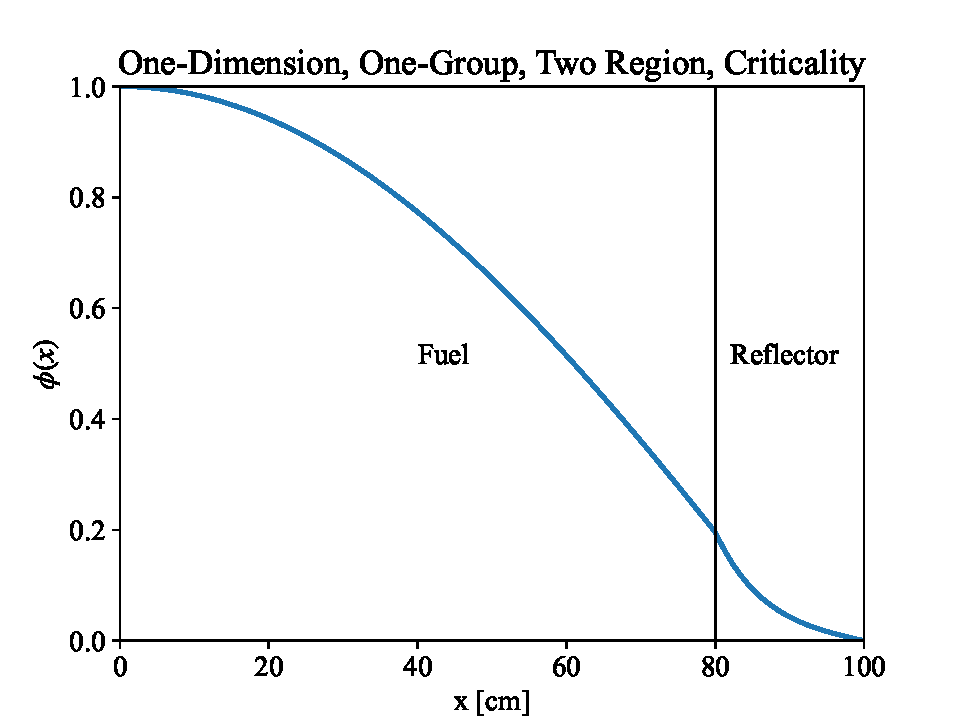
\includegraphics[width=0.7\textwidth]{2reg}
    \caption{Two Region Flux Shape.}
    \label{fig:2reg}
  \end{figure}

\section{Finite-Cylinder, One-Group, Criticality}
  \label{sec:deriv_finite_cyl}
  This three-dimensional problem can be simulated in three Cartesian dimensions 
  and, using symmetry, reduced to two cylindrical dimensions for simplified 
  analytic solution. This problem is located in $r \in [0,T]$ and $z \in [0,H]$
  where $r$ and $z$ are the radial and axial coordinates respectively. The
  material is homogeneous within the problem and has fixed coefficient
  properties. The diffusion equation for this problem is 
  \begin{equation}
    \label{eq:finite_cyl}
    -D \grad^2 \phi(r,z) + \Sigma_r \phi(r,z) = \frac{1}{\keff} \nu \Sigma_f
      \phi(r,z)
  \end{equation}
  with boundary conditions
  \begin{align}
    \label{eq:finite_cyl_bcz0}
    \phi(r,0) &= 0 ,\\
    \label{eq:finite_cyl_bczH}
    \phi(r,H) &= 0 ,\\
    \label{eq:finite_cyl_bcrT}
    \phi(T,z) &= 0 ,\\
    \label{eq:finite_cyl_bcr0}
    \phi(0,z) & \text{ is Finite}.
  \end{align}
  \eref{eq:finite_cyl} can be rewritten
  \begin{equation}
    \label{eq:finite_cyl_buckle}
    \grad^2 \phi(r,z) + B^2 \phi(r,z) = 0
  \end{equation}
  where $B$ is the buckling term and is given for this problem as
  \begin{equation}
    \label{eq:finite_cyl_b2}
    B^2 = \frac{\frac{1}{\keff} \nu \Sigma_f - \Sigma_r }{D}.
  \end{equation}
  The Laplacian in \eref{eq:finite_cyl_buckle} is expanded in two dimension
  cylindrical coordinates
  \begin{equation}
    \label{eq:finite_cyl_deriv}
    \frac{1}{r} \frac{\partial}{\partial r} \left( r \frac{\partial}{\partial r}
      \phi(r,z) \right) + \frac{\partial^2}{\partial z^2} \phi(r,z) + 
      B^2 \phi(r,z) = 0.
  \end{equation}
  Using the method of separation of variables, assume $\phi(r,z)$ is the product
  of two functions as
  \begin{equation}
    \label{eq:finite_cyl_separation}
    \phi(r,x) = R(r) \, Z(z).
  \end{equation}
  Inserting \eref{eq:finite_cyl_separation} into \eref{eq:finite_cyl_deriv}.
  \begin{align}
    \frac{1}{r} \frac{\partial}{\partial r} \left( r \frac{\partial}{\partial r}
      \left(R(r) Z(z) \right) \right) + \frac{\partial^2}{\partial z^2} \left(
      R(r) Z(z) \right) + B^2 \,R(r) \, Z(z) &= 0 \\
    Z(z) \frac{1}{r} \frac{\partial}{\partial r} \left( r
    \frac{\partial}{\partial r} R(r) \right) + R(r) \frac{\partial^2}{\partial
    z^2} Z(z) + B^2 \, R(r) \, Z(z) &= 0
  \end{align}
  Divide by the quantity $R(r)\,Z(z)$.
  \begin{equation}
    \label{eq:finite_cyl_sum}
    \frac{1}{R(r)} \frac{1}{r} \frac{d}{d r} \left( r
    \frac{d}{d r} R(r) \right) + \frac{1}{Z(z)}
    \frac{d^2}{d z^2} Z(z) + B^2 = 0
  \end{equation}
  Each of the derivatives operates on a function of only one variable, so the
  partial derivatives have become standard derivatives.

  The first two terms of \eref{eq:finite_cyl_sum} are function of only $r$ and
  $z$ respectively, and their sum is equal to a constant. Therefore, both of the
  terms must also be equal to a constant \cite{lamarsh1966}. Splitting
  \eref{eq:finite_cyl_sum} into two equations yields
  \begin{align}
    \label{eq:finite_cyl_radial_direction}
    \frac{1}{R(r)} \frac{1}{r} \frac{d}{dr} \left( r \frac{d}{dr} R(r) \right) +
      \beta^2 &= 0, \\
    \label{eq:finite_cyl_zeq}
    \frac{1}{Z(z)} \frac{d^2}{dz^2} Z(z) + \gamma^2 &= 0,
  \end{align}
  where
  \begin{equation}
    \label{eq:finite_cyl_b2_sum}
    B^2 = \beta^2 + \gamma^2.
  \end{equation}
  Beginning with the radial direction from
  \eref{eq:finite_cyl_radial_direction}.
  \begin{equation}
    \frac{1}{r} \frac{d}{dr} \left( r \frac{d}{dr} R(r) \right) + \beta^2 R(r) =
    0
  \end{equation}
  Multiplying by the radial coordinate $r$.
  \begin{equation}
    \frac{d}{dr} \left( r \frac{d}{dr} R(r) \right) + \beta^2 r = 0
  \end{equation}
  Noting the product rule of differentiation.
  \begin{equation}
    r \frac{d}{dr} R(r) + R(r) + \beta^2 R(r) = 0
  \end{equation}
  Dividing by the radial coordinate $r$.
  \begin{equation}
    \label{eq:finite_cyl_bessel}
    \frac{d}{dr} R(r) + \frac{1}{r} R(r) + \beta^2 R(r) = 0
  \end{equation}
  \eref{eq:finite_cyl_bessel} has general solution of the form
  \begin{equation}
    \label{eq:finite_cyl_bessel_general}
    R(r) = c_1 J_0(\beta r ) + c_2 Y_0(\beta r)
  \end{equation}
  where $J_0$ is the Bessel function of the first kind, zeroth order and $Y_0$
  is the Bessel function of the second kind, zeroth order. Requiring the flux to
  be finite at $r=0$ as per \eref{eq:finite_cyl_bcr0}.
  \begin{align}
    \lim_{r \rightarrow 0} Y_0(r) &\rightarrow - \infty, \\
    \label{eq:finite_cyl_c2}
    \therefore \; c_2 &= 0.
  \end{align}
  \eref{eq:finite_cyl_c2} is inserted into \eref{eq:finite_cyl_bessel_general}.
  \begin{equation}
    \label{eq:finite_cyl_j0}
    R(r) = c_1 J_0(\beta r)
  \end{equation}
  Evaluating the boundary condition at $r=T$ using \eref{eq:finite_cyl_j0} as
  specified in \eref{eq:finite_cyl_bcrT}.
  \begin{align}
    R(T) &= 0, \\
    &= c_1 J_0(\beta T).
  \end{align}
  For non-trivial $R(r)$, this is an eigenvalue problem. Then, $c_1$ is an
  arbitrary constant and the eigenmode is specified as
  \begin{align}
    \beta T &= \alpha_n \\
    \beta &= \frac{\alpha_n}{T} 
  \end{align}
  where $\alpha_n$ are the zeros of the $J_0$ function such that $J_0(\alpha_n)
  = 0$. The fundamental mode is given for $n=0$ as
  \begin{equation}
    \label{eq:finite_cyl_beta}
    \beta = \frac{\alpha_0}{T}
  \end{equation}
  where $\alpha_0$ is the first zero ($\alpha_0 \approx 2.4048$). Coefficient
  $c_1$ is arbitrary so allow $c_1 = R_0$. Then the solution for the function 
  $R(r)$ is
  \begin{equation}
    \label{eq:finite_cyl_R}
    R(r) = R_0 \, J_0\left(\frac{\alpha_0}{T} r\right).
  \end{equation}

  A similar process is repeated for $Z(z)$. The solution to $Z(z)$ is similar to
  the one-dimension, one-group, criticality problem presented in
  \sref{sec:deriv_1d1g}. This derivation is briefly repeated here. Recall
  \eref{eq:finite_cyl_zeq} which may be rewritten.
  \begin{equation}
    \frac{d^2}{dz^2} Z(z) + \gamma^2 Z(z) = 0
  \end{equation}
  which has general solution of the form
  \begin{equation}
    \label{eq:finite_cyl_z_general}
    Z(z) = c_3 \cos(\gamma z) + c_4 \sin(\gamma z).
  \end{equation}
  Evaluating \eref{eq:finite_cyl_z_general} at $z=0$ considering the boundary
  condition specified in \eref{eq:finite_cyl_bcz0}.
  \begin{align}
    Z(0) &= 0, \\
    &= c_3, \\
    \label{eq:finite_cyl_c3}
    \therefore \; c_3 &= 0.
  \end{align}
  Substituting \eref{eq:finite_cyl_c3} into \eref{eq:finite_cyl_z_general}.
  \begin{equation}
    \label{eq:finite_cyl_z_sin}
    Z(z) = c_4 \sin(\gamma z)
  \end{equation}
  Evaluating \eref{eq:finite_cyl_z_sin} at $z=H$ and considering boundary
  condition from \eref{eq:finite_cyl_bczH}.
  \begin{align}
    Z(H) &= 0, \\
    &= c_4 \sin(\gamma H).
  \end{align}
  For non-trivial $Z(z)$, the term $\sin(\gamma H)=0$ is required and $c_4$ is
  trivial and $\gamma$ specified by geometry as
  \begin{align}
    \gamma H &= n \pi, \\
    \gamma &= \frac{n \pi}{H}, \\
  \end{align}
  where $n$ is an integer. For the fundamental mode, $n=1$,
  \begin{equation}
    \label{eq:finite_cyl_gamma}
    \gamma = \frac{\pi}{H}.
  \end{equation}
  Coefficient $c_4$ is arbitrary so allow $c_4 = Z_0$. Then
  \begin{equation}
    \label{eq:finite_cyl_Z}
    Z(z) = Z_0 \sin\left(\frac{\pi}{H} z\right)
  \end{equation}

  \eref{eq:finite_cyl_R} and \eref{eq:finite_cyl_Z} are combined according to
  the separation of variables from \eref{eq:finite_cyl_separation}
  \begin{equation}
    \label{eq:analytic_finite_cyl}
    \phi(r,z) = \phi_0 \, 
      J_0\left(\frac{\alpha_0}{T} r\right) \sin\left(\frac{\pi}{H} z \right)
  \end{equation}
  where $\phi_0$ is arbitrary and $\phi_0 = R_0 Z_0$.
  An example flux plot for a slice of the cylinder is shown in 
  \fref{fig:finite_cyl}. Recall \eref{eq:finite_cyl_b2} and the form 
  \eref{eq:finite_cyl_b2_sum}. Coefficients $\beta$ and $\gamma$ are given in 
  \eref{eq:finite_cyl_beta} and \eref{eq:finite_cyl_gamma}. Then, an expression
  for $\keff$ can be constructed.
  \begin{equation}
    \label{eq:keff_finite_cyl}
    \keff = \frac{\nu \Sigma_f}{D \left( \left(\frac{\alpha_0}{T}\right)^2 +
    \left( \frac{\pi}{H}\right)^2 \right) + \Sigma_r}
  \end{equation}
  For $T = 50 \units{cm}$, $H = 100 \units{cm}$, and material cross sections
  specified in \tref{tab:finite_cyl_constants}
  \begin{equation}
    \keff = 0.996711
  \end{equation}
  
  The shape of the boundary as described by the discrete mesh is extremely 
  important for a circular (or curved) boundary. A simple example of this is 
  shown in \fref{fig:circle_meshes}. In a mesh refinement study, the mesh must 
  be regenerated with a halved mesh parameter, $h$, for each refinement, rather 
  than simply splitting nodes as splitting nodes would not improve the 
  description of the boundary.

  \begin{figure}
    \centering
    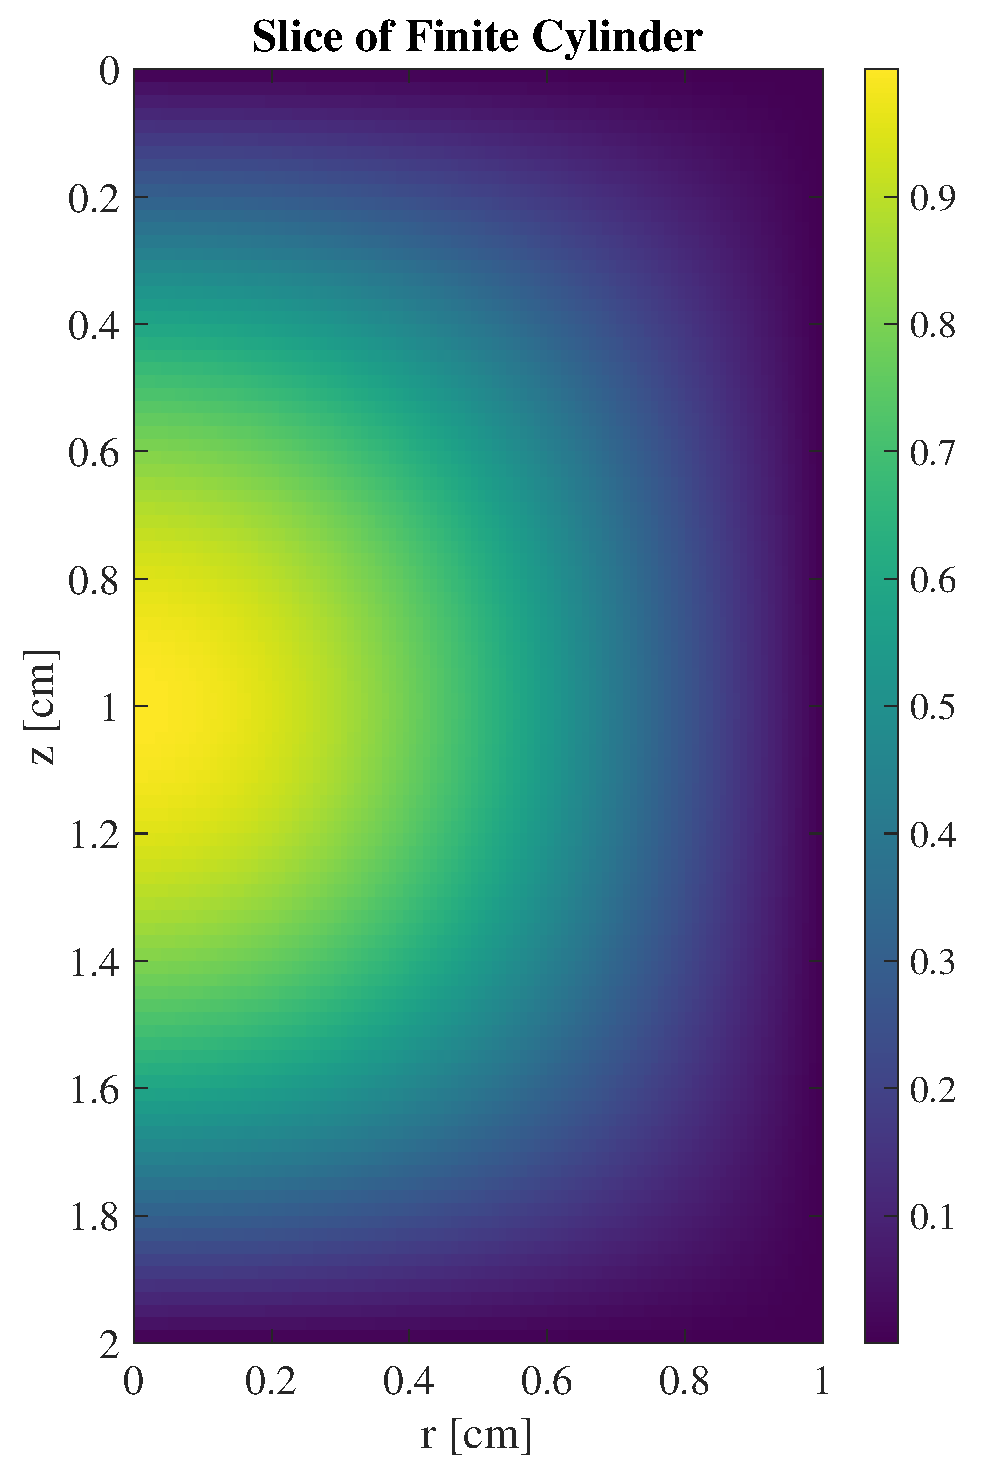
\includegraphics[width=0.4\textwidth]{finite_cyl}
    \caption{Example Finite Cylinder Flux Shape.}
    \label{fig:finite_cyl}
  \end{figure}

  \begin{figure}
    \centering
    \subfloat{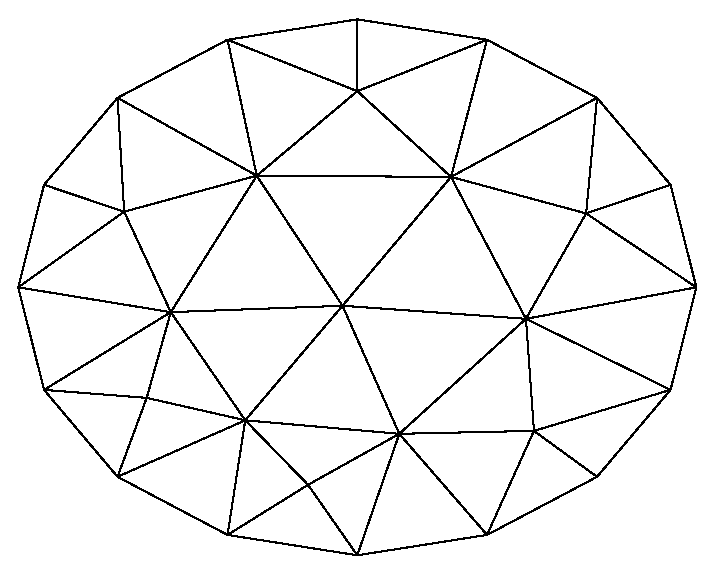
\includegraphics[width=0.35\textwidth]{cir0}}
    \vspace{0.2in}
    \subfloat{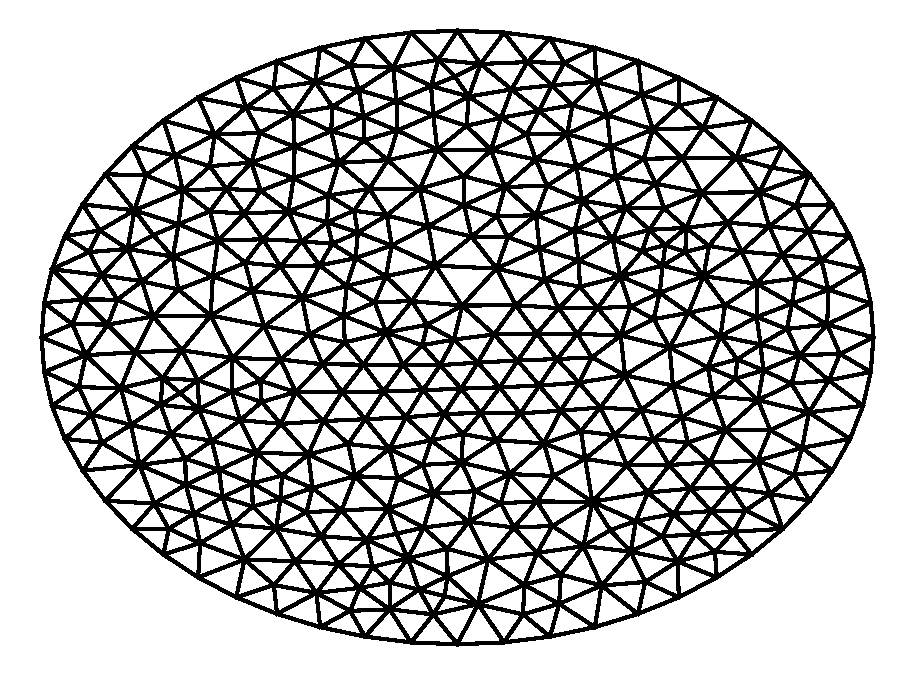
\includegraphics[width=0.35\textwidth]{cir2}}
    \caption{Mesh Refinement of Curved Mesh.}
    \label{fig:circle_meshes}
  \end{figure}

  \begin{table}
    \caption{Finite Cylinder Cross Sections.}
    \label{tab:finite_cyl_constants}
    \begin{center}
      \begin{tabular}{cc}
        \toprule
        Cross Section & Value \\
        \midrule
        $D \units{cm} $ & 1 \\
        $\Sigma_r \units{$\frac{1}{\text{cm}}$}$& 1 \\
        $ \nu \Sigma_{f} \units{$\frac{1}{\text{cm}}$} $ & 1 \\
        \bottomrule
      \end{tabular}
    \end{center}
  \end{table}

